\documentclass{beamer}
\usepackage[utf8]{inputenc}
\usepackage[T1]{fontenc}
\usepackage{ragged2e}
\justifying
 \title{Automatic exploit generation}
\author{Maxime, Manh-Dung, Tristan, Emilien, Gabriel + noms \\
\textbf{Supervision}: Jules - Facebook}
\institute{REDOCS 2020}
\date{\today}


\usetheme{Antibes}

\justifying
\setbeamertemplate{footline}[frame number]
\begin{document}

\begin{frame}
\titlepage
\end{frame}

\section*{Introduction}
\begin{frame}{Introduction}
\centering
Work given by Facebook
\end{frame}







\section{Problem overview}

\begin{frame}
\centering
\LARGE
Problem Overview
\end{frame}

\subsection{Context}

\begin{frame}{Context}

\begin{itemize}
\item Bugs in devices
\item Are they weaknesses ?
\end{itemize}
\begin{block}{Formal challenge}
Can we automatically turn static analysis reports into executable confirming the vulnerability of a program ?
\end{block}
\begin{figure}

\includegraphics[width = 2cm]{Figures/HeartbleedLogo.png}
\end{figure}

\end{frame}

\subsection*{Section example}
\begin{frame}{Section example}
\textit{Give an example of main.c with a bug}
We can show pictures or live performance. Ask the audience to detect the bug.
\end{frame}

\subsection{Infer tool}

\begin{frame}{Infer tool}

\begin{figure}

\includegraphics[width=10cm]{Figures/InferDrawing.png}
\end{figure}

\end{frame}

\begin{frame}

\begin{figure}

\includegraphics[width = 1.8cm]{Figures/InferLogo.png}

\end{figure}

\vspace{1cm}

\begin{itemize}
\item Static analysis tool from Facebook
\item \textbf{Capture} phase, then \textbf{Analysis} phase
\end{itemize}

\end{frame}

\begin{frame}{Infer tool example}

\textit{Give an example of our use of Infer on main.c}
We can show pictures or live performance.
\end{frame}

\subsection{Challenge approach}

\begin{frame}{Challenge approach}

\begin{figure}
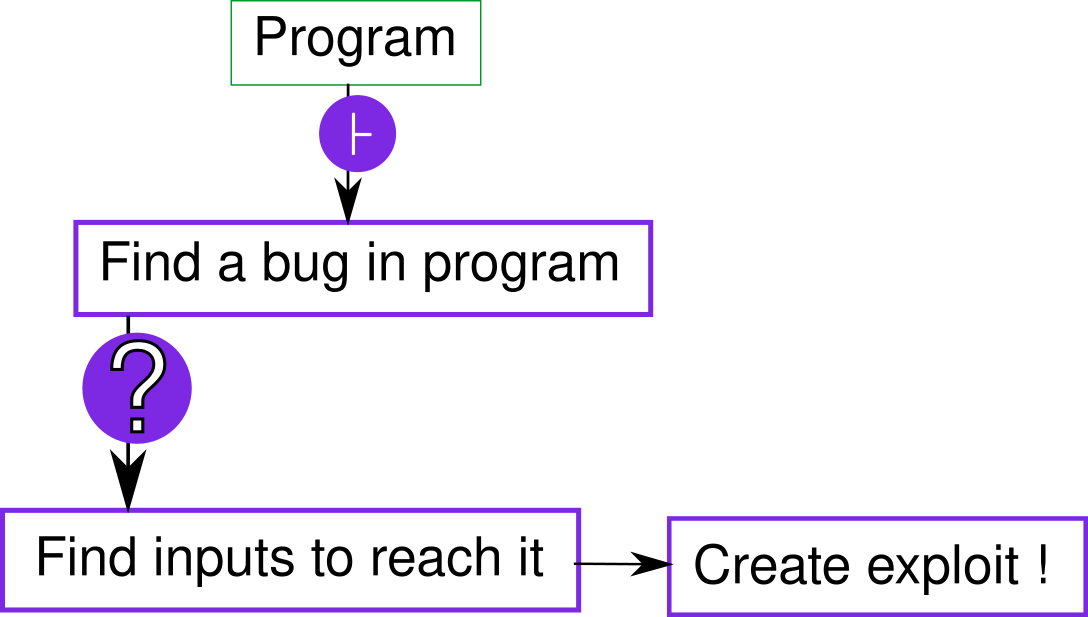
\includegraphics[width=8cm]{Figures/Workflow.png}
\end{figure}

\end{frame}


\begin{frame}{Challenge approach}

\begin{block}{Practical challenge}
Given the Infer information about bugs of a program A, create a program B that crashes A
\end{block}

\end{frame}

\begin{frame}{Table of content}
\tableofcontents
\end{frame}

\section{Proposed approaches}

\begin{frame}
\centering

Proposed approaches
\end{frame}



\subsection{Model checking}

\begin{frame}{Model checking}

Present model checking solution with Divine

\end{frame}


\subsection{SMT solvers/ SAT solver}

\begin{frame}{SMT / SAT solvers}

Present logic solvers

\end{frame}



\subsection{Fuzzing technique}

\begin{frame}{Fuzzing technique}

Present fuzzing techniques

\end{frame}

\begin{frame}{Fuzzing technique}

\begin{figure}
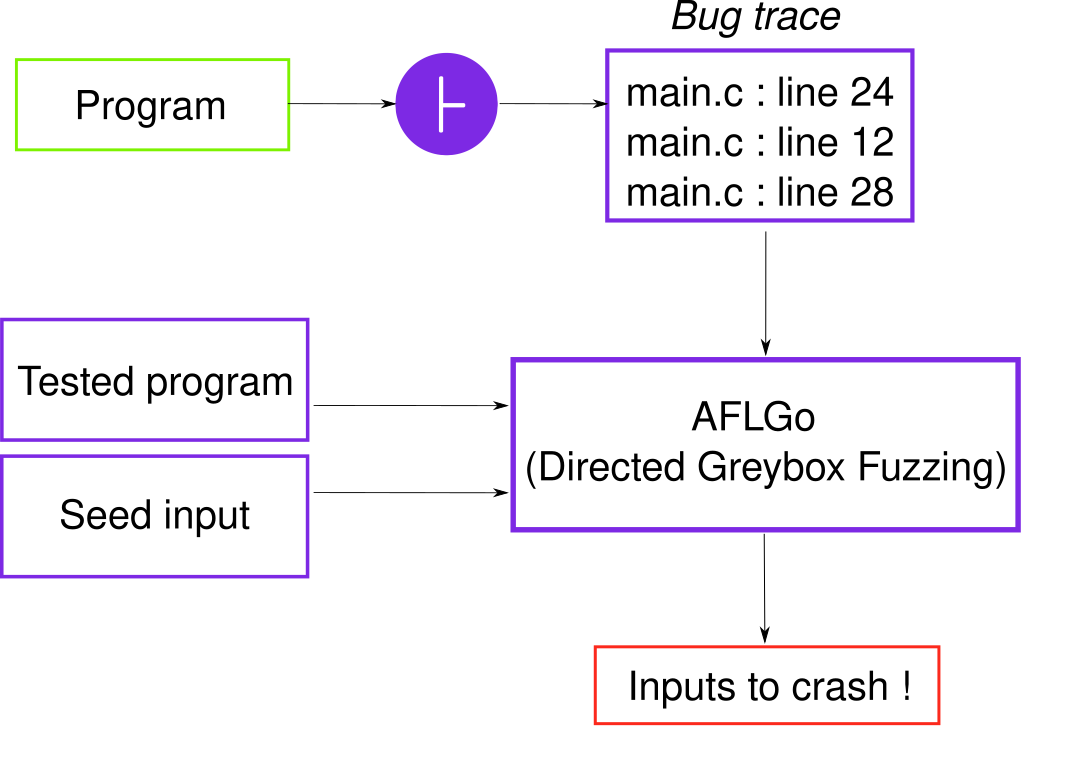
\includegraphics[width=8cm]{Figures/Fuzzing.png}
\end{figure}

\end{frame}


\section{Results and Future work}

\begin{frame}
\centering

Results and future work
\end{frame}

\subsection{Results}

\begin{frame}{Results}

\textit{Show a table approaches / program comparing results (yes/no, running time, implementation complexity, computational complexity } \\
\textit{Show some exploits results ?}

\end{frame}

\subsection{Future Work}
\begin{frame}{Future work}

Put eeeeeverything we think of. Ex
\begin{itemize}
\item Create a fully automatic process
\item Find automatic ways to generate exploits
\end{itemize}

\end{frame}


\begin{frame}{Thank you Questions ?}

See the title

\end{frame}

\end{document}
